%
% fourierkoef.tex -- Bestimmung der Fourier-Koeffizienten
%
% (c) 2018 Prof Dr Andreas Müller, Hochschule Rapperswil
%
\section{Fourier-Koeffizienten}
\rhead{Fourier-Koeffizienten}
In diesem Abschnitt
bestimmen wir die Fourierkoeffizienten für ein trigonometrisches Polynom
der Form
\begin{equation}
f(t)
=
a_0 + \sum_{k=1}^{n-1} a_k\cos kt + \sum_{k=1}^{n-1} b_k\sin kt + a_n\cos nt,
\label{skript:fourier:ansatz}
\end{equation}
so dass die Werte
\begin{equation}
y_j \quad\text{zu den Zeitpunkten}\quad t_j=2\pi\frac{j}{N},\qquad 1\le j< N
\label{skript:fourier:gleichungen}
\end{equation}
möglichst genau die Funktionswerte $f(t_j)$ reproduzieren.
Im Ansatz~\eqref{skript:fourier:ansatz} finden wir $2n$ zu bestimmende 
Koeffizienten, in \eqref{skript:fourier:gleichungen} finden wir dagegen
genau $N$ Gleichungen, mit denen wir die Koeffizienten bestimmen könnten.
Für $N>2n$ haben wir also zu viele Daten, für $N<2n$ reichen die Datenpunkte
nicht, die Koeffizienten zu bestimmen.
Im optimalen Fall, für $N=2n$ sollte es möglich sein, die Koeffizienten so
zu bestimmen, dass die Funktionswerte $y_j$ exakt reproduziert werden.

\subsection{Least Squares}
Für $N>2n$ können wir nicht erwarten, dass der Ansatz die Daten
exakt reproduzieren kann, wir müssen uns also mit einer
Näherungslösung begnügen.
Wir verlangen stattdessen, dass der Fehler der Lösung möglichst gering
wird, dass also
\[
L=L(a_0,a_1,\dots,a_n,b_1,\dots,b_{n-1})= \sum_{j=1}^N (y_j - f(t_j))^2
\]
möglichst klein wird.

Die Grösse $L$ wird minimal, wenn alle Ableitungen nach den Koeffizienten
verschwinden:
\[
\frac{\partial L}{\partial a_0}=0,
\qquad
\frac{\partial L}{\partial a_l}=0, \;{1\le l\le n}
\qquad
\frac{\partial L}{\partial b_l}=0, \;{1\le l\le n-1}
\]
Wir berechnen die Ableitungen:
\begin{align*}
\frac{\partial L}{\partial a_0}
&=
-2 \sum_{j=1}^N (y_j-f(t_j))\cdot \frac{\partial f}{\partial a_0}(t_j)=0
&&
\\
\frac{\partial L}{\partial a_l}
&=
-2 \sum_{j=1}^N (y_j-f(t_j))\cdot \frac{\partial f}{\partial a_l}(t_j)=0
&k&=1,\dots,n
\\
\frac{\partial L}{\partial b_l}
&=
-2 \sum_{j=1}^N (y_j-f(t_j))\cdot \frac{\partial f}{\partial b_l}(t_j)=0
&k&=1,\dots,n-1
\end{align*}
Man beachte, dass der erste Klammerausdruck in der Summe die Koeffizienten
$a_0$, $a_k$ und $b_k$ nur linear enthält.
Die Funktion $f$ enthält die Koeffizienten ebenfalls nur linear, so
dass die Ableitungsterme die Koeffizienten nicht mehr enthalten werden.
Tatsächlich ergibt die Berechnung der Ableitungen
\begin{align*}
\frac{\partial f}{\partial a_0}(t_j)
&=
1
&&
\\
\frac{\partial f}{\partial a_l}(t_j)
&=
\cos lt_j
&l&=1,\dots,n
\\
\frac{\partial f}{\partial b_l}(t_j)
&=
\sin lt_j
&l&=1,\dots,n-1
\end{align*}
Die Gleichungen, die wir lösen müssen, sind also
\begin{equation}
\begin{aligned}
0&=
\sum_{j=1}^N
\biggl(
y_j - a_0 - \sum_{k=1}^n a_k\cos kt_j \sum_{k=1}^{n-1} b_k\sin kt_j
\biggl)
\\
&=
\sum_{j=1}^N y_j
-Na_0
-\sum_{k=1}^n a_k \sum_{j=1}^N\cos kt_j
-\sum_{k=1}^{n-1} b_k \sum_{j=1}^N\sin kt_j,
\\
0&=
\sum_{j=1}^N
\biggl(
y_j - a_0 - \sum_{k=1}^n a_k\cos kt_j \sum_{k=1}^{n-1} b_k\sin kt_j
\biggl) \cos lt_j
\\
&=
\sum_{j=1}^N y_j \cos lt_j
-a_0\sum_{j=1}^N \cos lt_j
-\sum_{k=1}^n a_k \sum_{j=1}^N\cos kt_j\cos lt_j
-\sum_{k=1}^{n-1} b_k \sum_{j=1}^N\sin kt_j\cos lt_j,
\\
0
&=
\sum_{j=1}^N
\biggl(
y_j - a_0 - \sum_{k=1}^n a_k\cos kt_j \sum_{k=1}^{n-1} b_k\sin kt_j
\biggl) \sin lt_j
\\
&=
\sum_{j=1}^N y_j \sin lt_j
-a_0\sum_{j=1}^N \sin lt_j
-\sum_{k=1}^n a_k \sum_{j=1}^N\cos kt_j\sin lt_j
-\sum_{k=1}^{n-1} b_k \sum_{j=1}^N\sin kt_j\sin lt_j.
\end{aligned}
\label{skript:fourier:gl2}
\end{equation}
Hier haben wir die Faktoren $-2$ ebenfalls weggelassen.

\subsection{Trigonometrische Summen}
In den Gleichungen~\eqref{skript:fourier:gl2} treten trigonometrische Summen
der Form
\begin{equation}
\sum_{j=1}^N \cos kt_j
\qquad
\text{oder}
\qquad
\sum_{j=1}^N \sin kt_j,
\label{skript:fourier:trigosum}
\end{equation}
der Summen von Produkten wie
\begin{equation}
\sum_{j=1}^N \cos kt_j\cos lt_j,\quad
\sum_{j=1}^N \cos kt_j\sin lt_j
\quad
\text{oder}
\quad
\sum_{j=1}^N \sin kt_j\sin lt_j
\label{fourier:produkte}
\end{equation}
auf.
In diesem Abschnitt sollen diese Summen mit Hilfe einer geometrischen
Überlegung berechnet werden.

Wir befassen uns zunächst mit Summen der Form
\label{skript:fourier:trigosum} und beweisen den folgenden Satz.

\begin{figure}
\centering
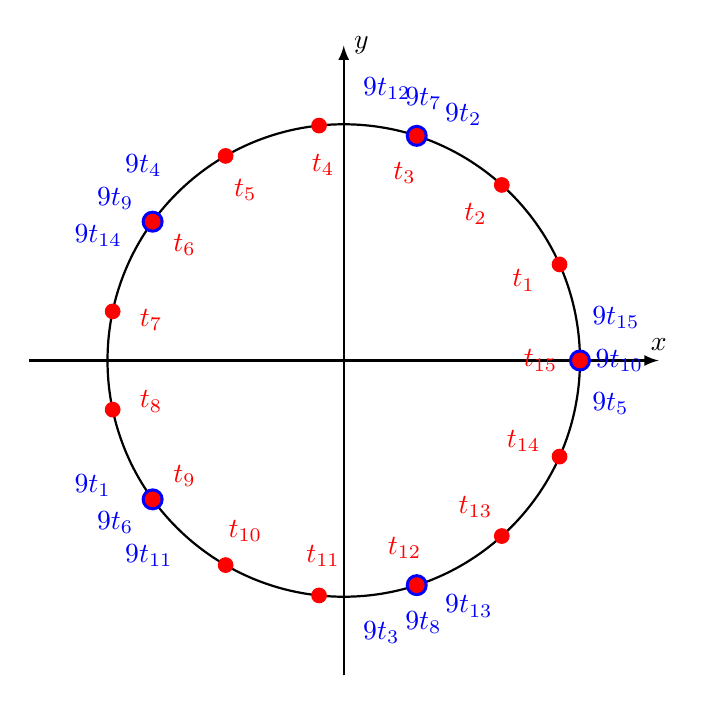
\begin{tikzpicture}[>=latex,thick]
\draw (0,0) circle[radius=3cm];
\draw[->] (-4,0)--(4,0) coordinate[label={$x$}];
\draw[->] (0,-4)--(0,4) coordinate[label={right:$y$}];
\foreach \j in {1,...,5}{
	\fill[color=blue] ({3 * cos(360 * \j/5)},{3 * sin(360 * \j/5)})
		circle[radius=0.14];
}
\def\N{15}
\foreach \j in {1,...,\N}{
	\fill[color=red] ({3 * cos(360 * \j/\N)},{3 * sin(360 * \j/\N})
		circle[radius=0.1];
	\node[color=red] at ({2.5*cos(\j*(360/\N))},{2.5*sin(\j*(360/\N))})
		{$t_{\j}$};
}
\def\k{9}
\pgfmathparse{\k*360/\N}
\xdef\a{\pgfmathresult}
\def\j{1}
\def\r{0.5}
\pgfmathparse{\j*\a-9}\xdef\aa{\pgfmathresult}
\node[color=blue] at ({3*cos(\aa)},{3*sin(\aa)})
	[shift={({\r*cos(\aa)},{\r*sin(\aa)})}] {$9t_{1\phantom{0}}$};
\def\j{2}
\pgfmathparse{\j*\a-9}\xdef\aa{\pgfmathresult}
\node[color=blue] at ({3*cos(\aa)},{3*sin(\aa)})
	[shift={({\r*cos(\aa)},{\r*sin(\aa)})}] {$9t_{2\phantom{0}}$};
\def\j{3}
\pgfmathparse{\j*\a-9}\xdef\aa{\pgfmathresult}
\node[color=blue] at ({3*cos(\aa)},{3*sin(\aa)})
	[shift={({\r*cos(\aa)},{\r*sin(\aa)})}] {$9t_{3\phantom{0}}$};
\def\j{4}
\pgfmathparse{\j*\a-9}\xdef\aa{\pgfmathresult}
\node[color=blue] at ({3*cos(\aa)},{3*sin(\aa)})
	[shift={({\r*cos(\aa)},{\r*sin(\aa)})}] {$9t_{4\phantom{0}}$};
\def\j{5}
\pgfmathparse{\j*\a-9}\xdef\aa{\pgfmathresult}
\node[color=blue] at ({3*cos(\aa)},{3*sin(\aa)})
	[shift={({\r*cos(\aa)},{\r*sin(\aa)})}] {$9t_{5\phantom{0}}$};
\def\j{6}
\pgfmathparse{\j*\a}\xdef\aa{\pgfmathresult}
\node[color=blue] at ({3*cos(\aa)},{3*sin(\aa)})
	[shift={({\r*cos(\aa)},{\r*sin(\aa)})}] {$9t_{6\phantom{0}}$};
\def\j{7}
\pgfmathparse{\j*\a}\xdef\aa{\pgfmathresult}
\node[color=blue] at ({3*cos(\aa)},{3*sin(\aa)})
	[shift={({\r*cos(\aa)},{\r*sin(\aa)})}] {$9t_{7\phantom{0}}$};
\def\j{8}
\pgfmathparse{\j*\a}\xdef\aa{\pgfmathresult}
\node[color=blue] at ({3*cos(\aa)},{3*sin(\aa)})
	[shift={({\r*cos(\aa)},{\r*sin(\aa)})}] {$9t_{8\phantom{0}}$};
\def\j{9}
\pgfmathparse{\j*\a}\xdef\aa{\pgfmathresult}
\node[color=blue] at ({3*cos(\aa)},{3*sin(\aa)})
	[shift={({\r*cos(\aa)},{\r*sin(\aa)})}] {$9t_{9\phantom{0}}$};
\def\j{10}
\pgfmathparse{\j*\a}\xdef\aa{\pgfmathresult}
\node[color=blue] at ({3*cos(\aa)},{3*sin(\aa)})
	[shift={({\r*cos(\aa)},{\r*sin(\aa)})}] {$9t_{10}$};
\def\j{11}
\pgfmathparse{\j*\a+9}\xdef\aa{\pgfmathresult}
\node[color=blue] at ({3*cos(\aa)},{3*sin(\aa)})
	[shift={({\r*cos(\aa)},{\r*sin(\aa)})}] {$9t_{11}$};
\def\j{12}
\pgfmathparse{\j*\a+9}\xdef\aa{\pgfmathresult}
\node[color=blue] at ({3*cos(\aa)},{3*sin(\aa)})
	[shift={({\r*cos(\aa)},{\r*sin(\aa)})}] {$9t_{12}$};
\def\j{13}
\pgfmathparse{\j*\a+9}\xdef\aa{\pgfmathresult}
\node[color=blue] at ({3*cos(\aa)},{3*sin(\aa)})
	[shift={({\r*cos(\aa)},{\r*sin(\aa)})}] {$9t_{13}$};
\def\j{14}
\pgfmathparse{\j*\a+9}\xdef\aa{\pgfmathresult}
\node[color=blue] at ({3*cos(\aa)},{3*sin(\aa)})
	[shift={({\r*cos(\aa)},{\r*sin(\aa)})}] {$9t_{14}$};
\def\j{15}
\pgfmathparse{\j*\a+9}\xdef\aa{\pgfmathresult}
\node[color=blue] at ({3*cos(\aa)},{3*sin(\aa)})
	[shift={({\r*cos(\aa)},{\r*sin(\aa)})}] {$9t_{15}$};

\end{tikzpicture}
\caption{Verteilung der Punkte $(\cos t_j, \sin t_j)$  auf dem Einheitskreis 
in rot.
Die Punkte $(\cos kt_j,\sin kt_j)$ für $k=9$ bilden eine Teilmenge, die
blau dargestellt ist.
Jeder blaue Punkt wird genau dreimal besucht, sie bilden ein gleichseitiges
Fünfeck mit den Punkten $(\cos 3t_j,\sin 3t_j)$ als Ecken.
Deren Schwerpunkt ist wieder der Nullpunkt.
\label{fourier:einheitskreis}
}
\end{figure}

\begin{satz}
\label{skript:fourier:orthogonalitaet1}
Für beliebige ganze Zahlen $l$, $0\le l\le n$, gilt
\begin{equation*}
\begin{aligned}
\sum_{j=1}^N \cos lt_j
&=
\begin{cases}
N&\qquad l=0\\
0&\qquad\text{sonst}
\end{cases}
\\
\sum_{j=1}^N \sin lt_j
&=0
\end{aligned}
\end{equation*}
\end{satz}

\begin{proof}[Beweis]
Wir betrachten zunächst den Fall $l=0$.
In diesem Fall ist $\sin lt_j=0$ und $\cos lt_j=1$ und damit
\[
\sum_{j=1}^N \cos lt_j = N
\qquad\text{und}\qquad
\sum_{j=1}^N \sin lt_j = 0.
\]
Im Folgenden können wir daher annehmen, dass $l\ne 0$.

In Abbildung~\eqref{fourier:einheitskreis} kann man sehen, dass die Punkte
$(\cos t_j,\sin t_j)$ auf dem Einheitskreis ein regelmässiges Polygon
bilden.
Der Schwerpunkt des Polygons ist ganz offensichtlich der Mittelpunkt.
Daraus folgt
\[
\sum_{j=1}^N \cos t_j = 0
\qquad\text{und}\qquad
\sum_{j=1}^N \sin t_j = 0.
\]
Damit ist der Satz für den Fall $l=1$ bewiesen.

Für beliebiges $l\ne 0$ beobachten wir, dass die Punkte 
$(\cos lt_j,\sin lt_j)$ eine Teilmenge der Punkte $(\cos t_j, \sin t_j)$
sind.
Wenn $l$ und $N$ teilerfremd sind, sind die Mengen gleich.
Wenn $l$ und $N$ dagegen den grössten gemeinsamen Teiler $r$ haben, dann
ist die Menge der Punkte $(\cos rt_j,\sin rt_j)$, ein regelmässiges
Polygon mit $2\pi / rt_1$ Ecken.
Diese Situation ist in Abbildung~\ref{fourier:einheitskreis} mit den
blauen Punkten für den Fall $r=3=\operatorname{ggT}(9,15)$
illustriert.
Wie im Falle von $l=1$ folgt, dass der Schwerpunkt des Polygons der
Nullpunkt ist, und damit, dass
\begin{align*}
\sum_{j=1}^N \cos lt_j 
=
\sum_{j=1}^N \cos rt_j 
=
0,
\\
\sum_{j=1}^N \sin lt_j 
=
\sum_{j=1}^N \sin rt_j 
=
0.
\end{align*}
Damit ist alles gezeigt.
\end{proof}

In \eqref{fourier:produkte} werden die Summen von Produkten benötigt.
Mit üblichen trigonometrischen Umformungen kann man diese in Summen
von einfachen trigonometrischen Funktionen umwandeln.
Wir verwenden dazu die Formeln
\begin{align}
\cos\alpha\cos\beta
&=
\frac12(\cos(\alpha-\beta)+\cos(\alpha+\beta)),
\label{fourier:coscos}
\\
\sin\alpha\cos\beta
&=
\frac12(\sin(\alpha-\beta) + \sin(\alpha+\beta)),
\label{fourier:sincos}
\\
\sin\alpha\sin\beta
&=
\frac12(\cos(\alpha-\beta) + \cos(\alpha+\beta)).
\label{fourier:sinsin}
\end{align}
Damit können wir die Summen in \eqref{fourier:produkte} umwandeln:
\begin{align*}
\sum_{j=1}^N \cos kt_j\cos lt_j
&=
\sum_{j=1}^N \frac12(\cos (k-l)t_j +\cos(k+l)t_j)
\\
&=
\frac12\sum_{j=1}^N \cos (k-l)t_j
+ \frac12\underbrace{\sum_{j=1}^N\cos(k+l)t_j}_{\displaystyle=0}
\\
&=
\begin{cases}
\displaystyle\frac{N}2&\qquad k=l\\
0&\qquad\text{sonst}
\end{cases}
\\
\sum_{j=1}^N \sin kt_j \sin lt_j
&=
\sum_{j=1}^N \frac12(\cos(k-l)t_j +\cos(k+l)t_j)
\\
&=\frac12\sum_{j=1}^N \cos(k-l)t_j
+\frac12\underbrace{\sum_{j=1}^N \cos(k+l)t_j}_{\displaystyle=0}
\\
&=
\begin{cases}
\displaystyle\frac{N}2&\qquad k=l\\
0&\qquad\text{sonst}
\end{cases}
\\
\sum_{j=1}^N \sin kt_j \cos lt_j
&=
\sum_{j=1}^N \frac12(\sin(k-l)t_j +\sin(k+l)t_j)
\\
&=
\frac12\underbrace{\sum_{j=1}^N \sin(k-l)t_j}_{\displaystyle=0}
+
\frac12\underbrace{\sum_{j=1}^N \sin(k+l)t_j}_{\displaystyle=0}
=0.
\end{align*}
Damit haben wir den folgenden Satz bewiesen:

\begin{satz}
Für beliebige $k,l\in \mathbb N$ gilt
\begin{align*}
\sum_{j=1}^N
\cos kt_j \cos lt_j
&=
\begin{cases}
N                     &\qquad k=l=0\\
\displaystyle\frac{N}2&\qquad k=l > 0\\
0                     &\qquad\text{sonst}
\end{cases}
\\
\sum_{j=1}^N
\sin kt_j \sin l_j
&=
\begin{cases}
\displaystyle \frac{N}2&\qquad k=l\\
0                      &\qquad\text{sonst}
\end{cases}
\\
\sum_{j=1}^N
\sin kt_j \cos lt_j
&=
0
\end{align*}
\end{satz}
In den folgenden Abschnitten verwenden wir diese Formeln, um die
Koeffizienten $a_k$ und $b_k$ zu bestimmen.
Der Koeffizient $a_0$ muss wegen des ersten Falles im Satz gesondert
behandelt werden.

\subsection{Bestimmung von $a_0$}
In der Gleichung
\[
0
=
\sum_{j=1}^Ny_j
-Na_0
-\sum_{k=1}^na_k\underbrace{\sum_{j=1}^N\cos kt_j}_{\displaystyle=0}
-\sum_{k=1}^nb_k\underbrace{\sum_{j=1}^N\sin kt_j}_{\displaystyle=0}
\]
verschwinden die Summen über $j$ und es bleibt die Gleichung
\begin{align*}
0
&=
\sum_{j=1}^Ny_j
-Na_0
\\
\Rightarrow\qquad
a_0&=\frac1{N}\sum_{j=1}^N y_j.
\end{align*}

\subsection{Bestimmung von $a_k, k>0$}
Zur Bestimmung von $a_k$ mit $k>0$ müssen wir die Gleichung
\[
0
=
\sum_{j=1}^N y_j\cos lt_j
-
a_0\underbrace{\sum_{j=1}^N\cos lt_j}_{\displaystyle=0}
-\sum_{k=1}^na_k\sum_{j=1}^N\cos kt_j\cos lt_j
-\underbrace{\sum_{k=1}^nb_k\sum_{j=1}^N\sin kt_j\cos lt_j}_{\displaystyle=0}
\]
heranziehen.
Die zweite und vierte Summe verschwindet, so dass wir die
die Gleichung
\begin{align*}
0&=
\sum_{j=1}^N y_j\cos lt_j
-\sum_{k=1}^na_k\sum_{j=1}^N\cos kt_j\cos lt_j
\end{align*}
erhalten.
Die innere Summe über $j$ verschwindet für alle Werte von $k$ ausser
für $k=l$, in diesem Fall ist sie $N/2$. 
Damit können wir nach $a_k$ auflösen:
\begin{align*}
0&=
\sum_{j=1}^N y_j\cos lt_j
-a_l\frac{N}2
\\
\Rightarrow\qquad 
a_l &= \frac{2}{N}\sum_{j=1}^Ny_j\cos lt_j.
\end{align*}


\subsection{Bestimmung von $b_k$}
Zur Bestimmung von $b_k$ müssen wir die Gleichung
\[
0=\sum_{j=1}^N y_j\sin lt_j 
-a_0\sum_{j=1}^N \sin lt_j
-\sum_{k=1}^na_k\sum_{j=1}^N\cos kt_j\sin lt_j
-\sum_{k=1}^nb_k\sum_{j=1}^N\sin kt_j\sin lt_j
\]
heranziehen.
Die zweite und die dritte Summe verschwindet und in der letzten Summe
verschwinden alle Terme ausser der Term mit $k=l$, für den die
innere Summe den Wert $N/2$ hat.
Damit wird die Gleichung vereinfacht zu
\begin{align*}
0
&=
\sum_{j=1}^Ny_j\sin lt_j - b_l\frac{N}2
\\
\Rightarrow\qquad
b_l
&=
\frac{2}{N}\sum_{j=1}^Ny_j\sin lt_j.
\end{align*}

\subsection{Zusammenstellung der Resultate}
Sei $N=2n$ eine gerade natürliche Zahl.
Eine $2\pi$-periodische Funktion $f(t)$ kann als trigonometrisches Polynom
der Form
\[
p(t)
=
a_0 + \sum_{k=1}^{n-1} (a_k\cos kt + b_k\sin kt) + a_n\cos nt
\]
derart approximiert werden, dass zu den Zeiten $t_j=2\pi j/N, j=1,\dots,N$ 
die Funktion und das trigonometrische Polynom übereinstimmen:
\[
p(t_j) = y_j = f(t_j).
\]
Dazu müssen die Koefizienten
\begin{align*}
a_0
&=
\frac{1}N
\sum_{j=1}^N y_j
\\
a_k
&=
\frac{2}N
\sum_{j=1}^N y_j\cos t_j
=
\frac{2}N
\sum_{j=1}^N y_j\cos \frac{2\pi j}{N}&k&=1,\dots,n
\\
b_k
&=
\frac{1}N
\sum_{j=1}^N y_j\sin t_j
=
\frac{2}N
\sum_{j=1}^N y_j\sin \frac{2\pi j}{N},&k&=1,\dots,n-1
\end{align*}
verwendet werden.


\subsection{Beispiel: Dreiecksfunktion}
\begin{figure}
\centering
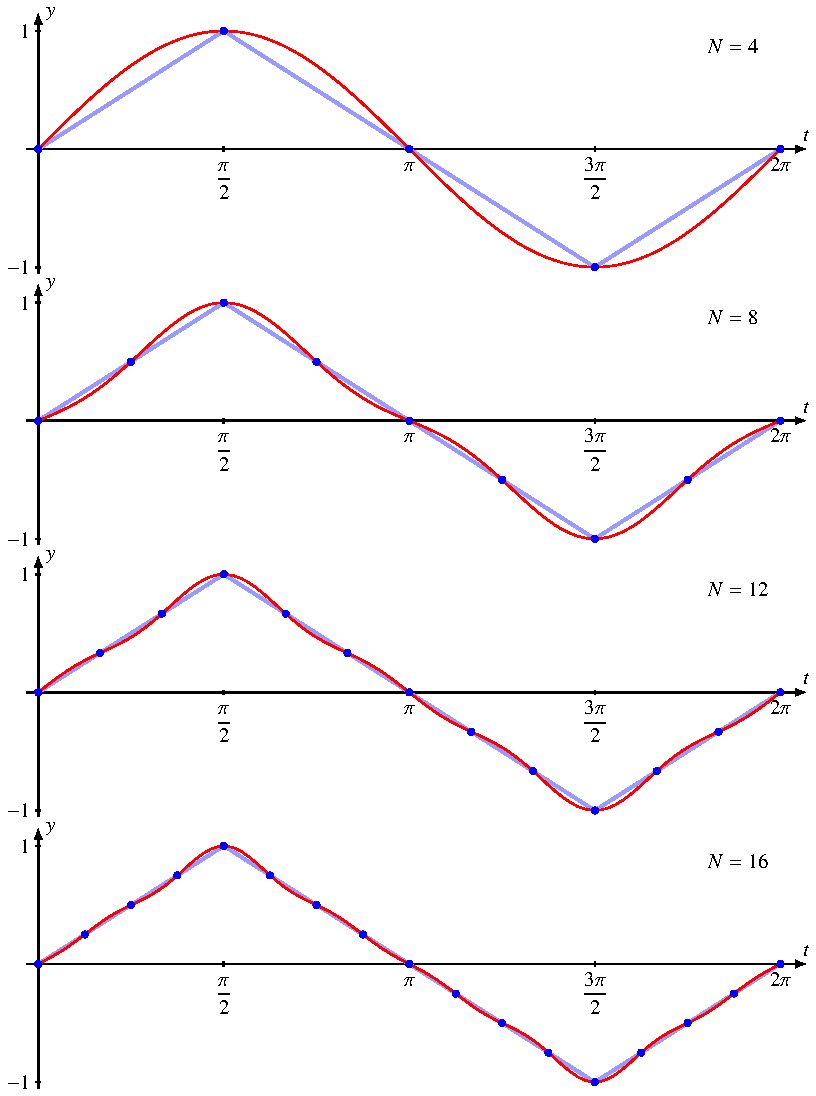
\includegraphics{chapters/6/dreieck.pdf}
\caption{Dreiecksfunktion approximiert mit trigonometrischen Polynomen 
mit verschiedenen Werten von $N$.
\label{skript:fourier:beispiel}}
\end{figure}
\begin{table}
\centering
\setlength{\tabcolsep}{5pt}
\begin{tabular}{>{$}l<{$}>{$}r<{$}>{$}r<{$}>{$}r<{$}>{$}r<{$}>{$}r<{$}>{$}r<{$}>{$}r<{$}>{$}r<{$}}
&N=4&N=8&N=12&N=16&N=20&N=24&\dots&N=\infty\\
\hline
b_1&1& 0.85355& 0.82934& 0.82107& 0.81727& 0.81522&& 0.8105695\\
b_3& &-0.14645&-0.11111&-0.10124&-0.09704&-0.09484&&-0.0900633\\
b_5& &        & 0.05954& 0.04520& 0.04000& 0.03748&& 0.0324228\\
b_7& &        &        &-0.03249&-0.02519&-0.02207&&-0.0165422\\
b_9& &        &        &        & 0.02050& 0.01627&& 0.0100070\\
b_{11}&&      &        &        &        &-0.01413&&-0.0066989\\
%\hline
\end{tabular}
\caption{Nicht verschwindende Fourier-Koeffizienten der
Dreiecksfunktion~\eqref{skript:fourier:dreieck}
für verschiedene Werte von $N$.
In der Spalte ganz rechts unter $N=\infty$ die Werte für die
Fourierkoeffizienten der stetigen Fourier-Reihe
nach \eqref{fourier:normalekoeffizienten}.
\label{skript:fourier:dreieckkoef}}
\end{table}
Als Beispiel untersuchen wir die Approximation der
$2\pi$-periodischen Dreiecksfunktion, die auf dem Interval $[0,2\pi)$
durch
\begin{equation}
f(t)
=
\begin{cases}
\displaystyle t\cdot\frac{2}{\pi}    &\displaystyle \qquad 0\le t < \frac{\pi}2\\
\displaystyle 2-t\cdot\frac{2}{\pi}  &\displaystyle \qquad \frac{\pi}2\le t < \frac{3\pi}2\\
\displaystyle t\cdot\frac{2}{\pi} - 4&\displaystyle \qquad \frac{3\pi}2\le t <2\pi
\end{cases}
\label{skript:fourier:dreieck}
\end{equation}
gegeben ist,
mit Hilfe eines trigonometrischen Polynoms.
In Abbildung~\ref{skript:fourier:beispiel} ist die Dreiecksfunktion
hellblau dargestellt.

Weil die Funktion antisymmetrisch ist, verschwinden alle $a_k$-Koeffizienten.
Da die Funktion ausserdem symmetrisch ist bezüglich $\frac{\pi}2$ verschwinden
alle geraden $b_k$-Koeffizienten.
Für $N=4$ besteht $y$ nur aus vier Werten: $1$, $0$, $-1$ und $0$,
in diesem Fall muss die Funktion mit nur einem einzigen $\sin$-Term
mit dem Fourier-Koeffizienten $b_1$ darstellbar sein.
Tatsächlich ist $f(t) = \sin t$ an den Stellen $t_j=2\pi j/4$, $j=1,\dots,4$
(blau in Abbildung~\ref{skript:fourier:beispiel}),
dies wird in Abbildung~\ref{skript:fourier:beispiel} ganz oben gezeigt.
Erhöht man $N$, wird die Approximation immer besser, dies zeigen die
weiteren Graphiken in Abbildung~\ref{skript:fourier:beispiel}.

Die Berechnung der Fourier-Koeffizienten mit den Integralformeln
\eqref{fourier:normalekoeffizienten}
liefert für die Dreiecksfunktion~\eqref{skript:fourier:dreieck}
die Formel
\[
b_k = (-1)^{(k-1)/2}\frac{8}{\pi^2k^2}
\]
für ungereade Werte von $k$.
Diese Werte sind in der letzten Spalte unter $N=\infty$ dargestellt.
Für zunehmendes $N$ konvergieren die diskreten Koeffizienten $b_k$ gegen 
diese stetigen Werte.

